% define a neural network and the classification problem
% usually a sdg approach is chosen; works fine
% is performs optimization of a loss function
% question: how does the loss function geometry looks like?
% what is the dependence between data geometry, nn architecture and loss geom?
\documentclass{article}
\usepackage{comment}
\usepackage{amsmath}
\usepackage{amssymb}
\usepackage{graphicx}

\title {Geometry of the good local minima in a Neural Network loss function}

\begin{document}
\maketitle

To train a Neural Network (abbreviated "nn") means to minimize a specific
map called the loss function. Modern techniques like sgd often reach
the goal, but suffer from local minima that can spoil the
optimization process. Knowing the geometry of these can help
avoiding such pitfalls. 


In this informal report, I describe
how I (partially) studied the geometry of loss functions for very small nn
and highlight pros and cons of such a method. Ideally, I would like
to clarify the relation between the geometry of the dataset, the 
architecture of the network and the resulting geometry of the loss map.


\section{Basic setting}
Given a set of $10$ point on the square $[-1, 1]^2$ subdivided into two
categories ($1$ and $0$), 
I want to train a small neural network to classify the points 
correctly, i.e. such that for each point in input it returns the right
label as output.
The nn is formally seen as 
$\mathbb{R}^2 \to \mathbb{R}^2$ composed with a softmax function 
to bring the values into $0$ or $1$. This structure is constant for
the whole report, and the only change is made in the nn architecture.
For instance, a notation like $[2, 3, 4]$ 
means that the network has three hidden layers:
the first with $2$ neurons, the second with $3$ and the last with $4$. 
The input and the output layers always
have $2$ neurons, and the network is always finally composed with the 
softmax function.


This classification 
problem on small nn and data is straightforward, 
easily solvable by using common sgd.
On the other hand, the more complex the dataset and the nn architecture are,
the harder the problem becomes. 
Classic sgd might fail or
be too slow. The reason is known: the loss function suffers multiple 
local minima that prevent the optimization to be successful.


Therefore the motivation: by increasing the understanding of the
loss function geometry, for instance knowing where good minimization
points are expected to be found, one could potentially discover a way to
boost optimization.


As a first step, I assumed to work with very simple nn models
and an easy dataset.
In the next section, I explain how I approximated the geometry
of the corresponding loss functions.


\section{Geometry of the loss function}
If the neural network has $p$ parameters (weights and biases), then
the loss function to minimize (to successfully train the network)
is a map $U : \mathbb{R}^p \to \mathbb{R}$ with a specific form of
choice (binary entropy in my case).
Practical experience suggests that the domain can be restricted to 
a hypercube $[-L, L]^p$, say of length $L = 10$. Since I am interested
in studying convexity properties, I replaced the loss with $e^{-U}$ and
saw it as a probability density on the hypercube. Then, I used a MCMC
approach to sample from it. As a consequence, 
the set of the Markov chain samples composes an approximation
of the probability density function, 
which (up to $e^{-(\cdot)}$) is precisely the loss function "plot"
I am interested in.


It sound good in theory, but since the number $p$ of the
network parameters become easily very big ($15 < p < 2.000.000$), 
the probability distribution 
to sample from is very high dimensional making the
procedure hard and partially impractical.
That said, I temporarily ignored this issue and
adopted a naive and simple Random Walk MC: it converges very slow, but it's
cheap since it does not require any gradient evaluation. In principle,
this step can be improved since for any nn, "gradient = backward propagation",
known to be relatively convenient. For the moment, instead of going in that
direction, I customized the algorithm in order to exploit CPU (and not GPU)
parallelization, making each simulation manageable in around $1$ day.
I "verified" convergence by always running multiple chains and taking their
expectation values, considering enough when they distributed
according to a Gaussian (i.e. when they entered the CLT regime).


Summing up: the complete geometry of the $p$-dimensional
loss function is obtained by running
a Monte Carlo algorithm, whose performance have margins of improvements.


\section{Good local minima: dimension reduction from $p$ to $2$}
In the previous section I explained how I obtained
set of samples capable of reconstructing the geometry of
the loss function $U : \mathbb{R}^p \to \mathbb{R}$.
Coming from a Markov chain, they are a collection of arrays
(e.g. $\sim 20.000$), each of dimension $p$ (e.g. $\sim 20$).


To use them effectively, the domain of data visualization comes into play.
I tried many classical Machine Learning techniques, but I was particularly
surprised by the kernelized PCA method with an RBF kernel.


I didn't implement it by my own, rather I used the prebuilt in the sklearn
Python3 module. When reducing the dimension from $p$ to $3$
(to visualize with eyes) I obtained a very low
($< 0.01$) approximation error! 


Recall that I am interested in understanding where \emph{all} 
the minimal points of
$U$ are located. By combining clustering techniques with gradient descent,
I found that the number of generic local minima is generally huge and
difficult to manage. Instead, I decided to only focus on "good" local minima,
i.e. local minima having a low loss value and leading therefore
to a good model training. Since the goal of every optimization algorithm
is basically to reach at least one of them, understanding their
space distribution might be helpful anyway.


Given the 3D reduction just described, I selected all the good local
minima by just taking the points where the loss map was low enough ($< 0.1$);
this is of course imprecise, but suffices as a first idea.
Indeed, most of them seemed to lie on a 2D hyperplane!
I verified it by running a standard linear PCA that always confirmed
this impression giving variance expression around $0.9$ (max is $1.0$),
which is very good!


Summing up, I noticed in a first experiment (details omitted) that: given a nn, 
the points of minimization leading to good training results
are located on a low-dimensional hyperplane detectable by using compositions
of kernel/linear PCA transformations.


Then, this fact happened again with various further experiments,
so I decided to start a systematic analysis trying to relate
the unexpected "hyperplane arrangement of minima", to the geometry
of the dataset under analysis, to the architecture of the neural network.
My first experiments are described below.


\section{First experiments and results}
First of all, I fixed a set of $10$ point in $[-1, 1]$ with random
(then fixed) labels.
I set a neural network architecture of type $[2, 2]$ having a total
of $p = 18$ parameters, and I restricted the loss function $U$ on hypercubes
$[-10, 10]^{18}$.


Then, I performed three experiments: all following the same exact procedure,
except for having a different value of $\theta = 0, 120, 240$ as now described.


Each experiment consists in the following steps:
\begin{enumerate}
	\item fix $\theta$ to $0, 120$ or $240$
	\item rotate the dataset above with angle $\theta$: plot the points;
	\item run a MC complete simulation to reconstruct the shape of $U$,
		(a $18$-dimensional object) i.e. the loss function of interest;
	\item "check" convergence by looking at the marginals of the
		expectations of the MC chains: if they are gaussians (and
		they almost always were),
		trust the results and proceed;
	\item collect $~20.000$ chain samples (each being of dimension
		$18$) and reduce their dimension to $3$ by using
		the kernel PCA (rbf) offered with sklearn;
	\item select only the points with energy below $0.1$, and reduce them
		in $2D$ by using linear PCA. If all the error approximations
		are good enough (they always were), plot the points.
\end{enumerate}


For each experiment I included two plots, for a total of six.
Three plots refer to the dataset to classify, always the same except from the
rotation by $\theta$, and three to the resulting $2D$ reduction of the 
loss function good local minima.


In other words, I am trying to answer to the question:
seen that the dimensionality reduction trick seem to work
with all the three experiments, how does the rotation of the points
afflict the geometry of the useful local minima in the loss function?
The answer is provided by the plots: nothing seems to change.

\begin{figure}
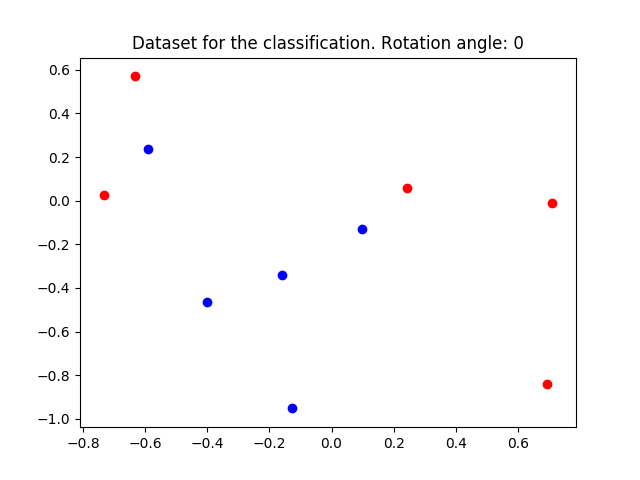
\includegraphics[width=0.7\textwidth]{../theta0/points_wseed2angle0.png}
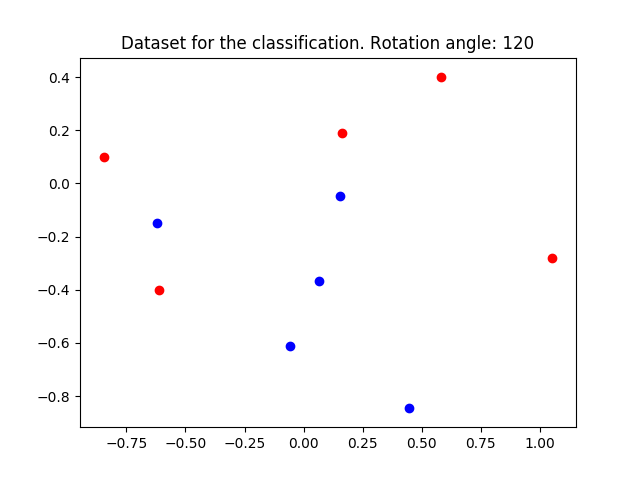
\includegraphics[width=0.7\textwidth]{../theta120/points_wseed2angle120.png}
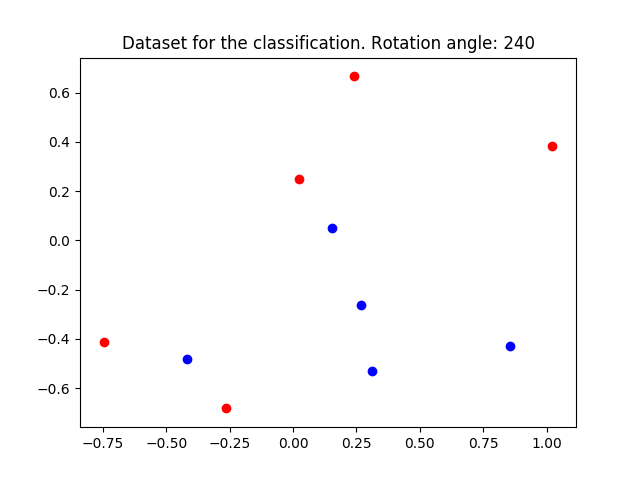
\includegraphics[width=0.7\textwidth]{../theta240/points_wseed2angle240.png}
	\caption{The dataset for each experiment. The points are always
	the same, expect for being rotated by and angle theta. The two 
	colors represent the two classes.}
\end{figure}


\begin{figure}
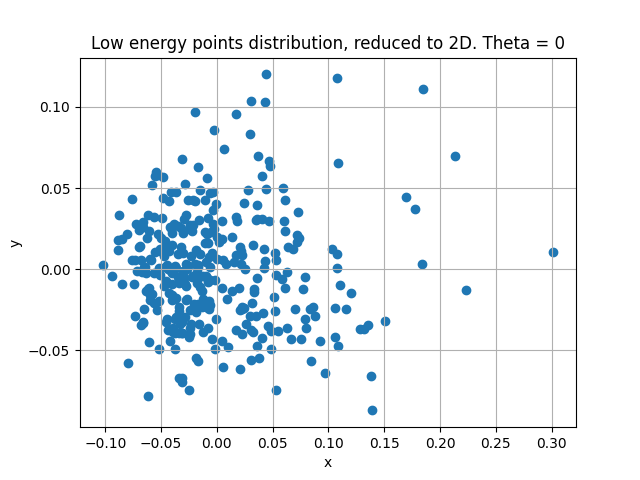
\includegraphics[width=0.7\textwidth]{../theta0/reduction2D.png}
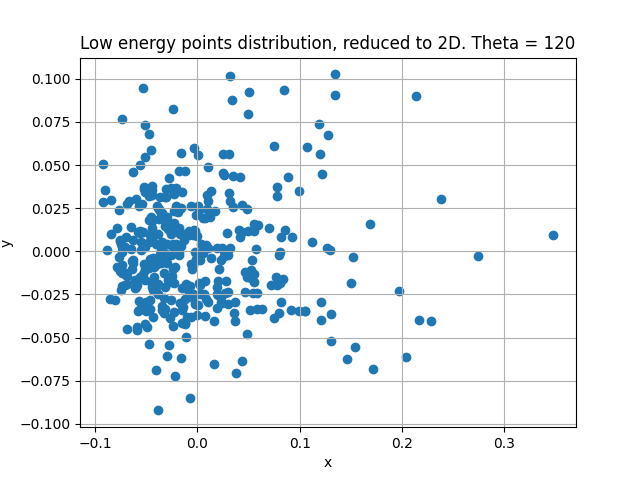
\includegraphics[width=0.7\textwidth]{../theta120/reduction2D.png}
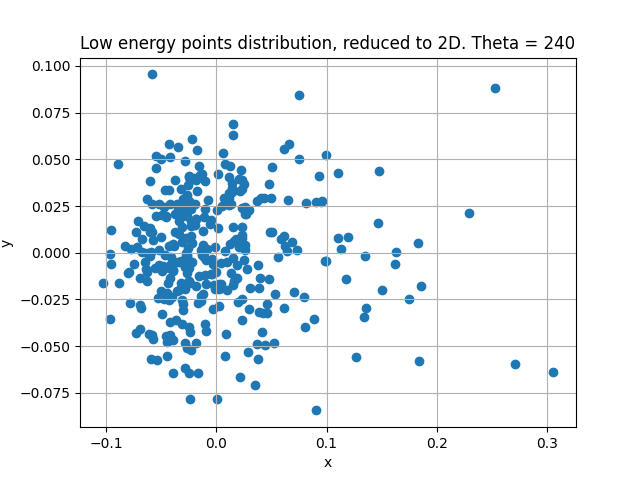
\includegraphics[width=0.7\textwidth]{../theta240/reduction2D.png}
	\caption{Roughly speaking, a 2D plot of the
	local minima having good training properties.
	Despite	the dataset are rotated, they stay the same.}
\end{figure}

\section{Conclusion}
The experiments above shown cases where the geometry of the dataset
does not to seem to influence the geometry of part of the loss function,
at least the distribution of local minima with good classification
properties. 


Furthermore, the mere fact that they lie so well in a hyperplane
can provide motivation in experimenting more.
For instance, new improvements that can be done are:
\begin{itemize}
	\item replace the Random Walk with a more efficient MC (HMC?);
	\item replace CPU parallelization with GPU parallelization;
	\item allow more generic transforms on the dataset;
	\item modify the neural network architecture;
	\item try to characterize \emph{all} the local minima,
		instead of only the good ones;
\end{itemize}

Unfortunately, all my observations must be considered to be 
very theoretical.
Indeed, the MC technique here used cannot be used for realistic dataset. 
For instance, I tried with the common MNIST classification
using a simple convolutional neural network, but the number
of parameters, i.e. the dimension of the loss function
was prohibitive. Not only I had performance issue,
but I not even had enough computer memory (RAM as well as
HDD) to store the Markov Chain samples ($20.000$ in total,
each being an array of dimension $> 100.000$).


\end{document}
